\chapter{Inter-Island Governmental Organisation (IIGO)}


The role of IIGO is to maintain, update, and revise the rules concerning provision to managing the long-term collective risk dilemma (ltCRD).

\begin{itemize}
    \item There will be 3 distinct branches in the IIGO: the \textbf{legislative branch}, \textbf{executive branch} and \textbf{judicial branch}\footnote{This is, as no surprise, inspired by the separation of powers in Western democracies.}.
    \item Each role is put in power according to the  transfer-of-power rules (see Section~\ref{subsec:transfer-of-power} for more detail).
    \item The head of the legislative branch is the Speaker, the head of the executive branch is the President, and the head of judicial branch is the Judge.
    \begin{itemize}
        \item  The Speaker, President and Judge are selected, through a democratic election, from the islands in the archipelago\footnote{This naming is inspired by the roles in the US Government.}.
        \item The resources gathered by the archipelago are endogenous, hence acting on the institutional powers granted to the Speaker, President or Judge costs resources.
        \item For their duty, the President, the Speaker and the Judge receive a salary for each of their turns in office (see Section~\ref{subsec:salary} for more detail).
        \item The limit of the powers of the President, Speaker and Judge are defined in this chapter (e.g. the Speaker can only call one vote per turn).

    \end{itemize}
\end{itemize}

\subsection{IIGO Specific Definitions}
\begin{definition} \label{def:ballot}
    A \textbf{ballot} is related to each island's \textbf{power} to support or disagree with the rule specified in the vote called by the President and to vote in favour or against an island for a specific role (i.e. the President, Speaker, Judge) at each round of the game.
\end{definition}


%\begin{definition} \label{def:vote}
    %A \textbf{vote} is related to a role's (i.e. the President, Speaker, Judge) \textbf{power} to call a vote for a specific rule or an election.
%\end{definition}


\begin{definition} \label{def:tax}
    The \textbf{taxation} is related to the President's \textbf{power} to request a specific \underline{\textbf{minimum}} amount of contribution from each island to the common pool at each round of the game.
\end{definition}

\begin{definition} \label{def:alloc_req}
    An \textbf{allocation request} is related to each island's \textbf{power} to request a specific amount of resource allocation from the President at each round of the game.
\end{definition}


\begin{definition} \label{def:rule_prop_list}
A \textbf{rule proposal list} is related to each island's \textbf{power} to propose a specific rule to be passed to the President at each round of the game.
\end{definition}

\begin{definition} \label{def:invst}
    An \textbf{investigation} is related to the Judge's \textbf{power} to acquire information to make a decision, followed by a calculation of the expected results and checking whether some specific rules have been obeyed, exclusively for the actions carried out by the \textbf{islands}.
\end{definition}


An example of an \emph{investigation}: The President has permitted the island $X$ to take the amount of $Y$ resources from the common pool. Upon \emph{investigation} carried out by the Judge, it is revealed that the amount of resources taken out from the common pool by the island $X$ is, in fact, $Y'$ such that $Y' \neq Y$.


\begin{definition}
\textbf{Monitoring} is a government official's \textbf{power} to perform event recognition and to check whether some specific rules have been obeyed.
\end{definition}

An example of \emph{monitoring}: The Speaker has performed only the following action: \emph{counted the votes and calculated the result} for a rule. Upon \emph{monitoring} carried out by the President, it is noticed that the Speaker has not made any \emph{announcement}. Hence, the Speaker has not followed their obligation to \emph{announce} the result of any vote held.

See Section~\ref{sec:accountability} for more information about which roles can monitor which ones.


\begin{definition}
\textbf{Investigative-monitoring} is a government official's \textbf{power} to acquire the information used in acting on a governmental power followed by calculation of the expected results and checking whether some specific rules have been obeyed, exclusively for the actions carried out by a government official they are responsible for.
\end{definition}

An example of \emph{investigative-monitoring}: The Speaker has performed the following actions: \emph{counted the votes and calculated the result $R$} for a vote $V$ and \emph{announced} the result $R'$ for the vote $V$. Upon \emph{investigative-monitoring} carried out by the President, it is noticed that $R' \neq R$. Hence, the Speaker has modified the announced result.


\begin{definition}
The \textbf{sanction} is related to the Judge's \emph{power} to punish non-compliant islands when their disobedience is confirmed through investigations at a specific turn.
\end{definition}


\begin{definition}
The (judicial) \textbf{pardon} is related to the Judge's \emph{power} to forgive a non-compliant island at a specific turn.
\end{definition}

\begin{definition}
The \textbf{budget} is the maximum amount of resources a role is permitted to spend from the common pool as it performs its own institutional-power-enabled actions at a specific turn.
\end{definition}


\begin{definition}
The \textbf{salary} is the amount of resources a role is to be given from the common pool as a reward for performing its institutional-power-enabled actions at a specific turn.
\end{definition}

\begin{definition} \label{def:term}
A \textbf{term} is the number of turns an island is \emph{permitted} to hold a role, and after which the responsible role (indicated in the transfer-of-power cycle in Figure~\ref{fig:cycles_in_IIGO}) is \emph{obliged} to initiate transfer-of-power.
\end{definition}

\subsection{\emph{Power}, \emph{Permission} and \emph{Obligation} Distinction}
In the rest of the specifications, we will be specifically using the following three terms to define the actions and responsibilities carried out by the Speaker, President, Judge (see Figure~ \ref{fig:per_obl_sets}):
\begin{itemize}
    \item Power
    \item Permission
    \item Obligation
\end{itemize}



\begin{figure}[H]
\centering
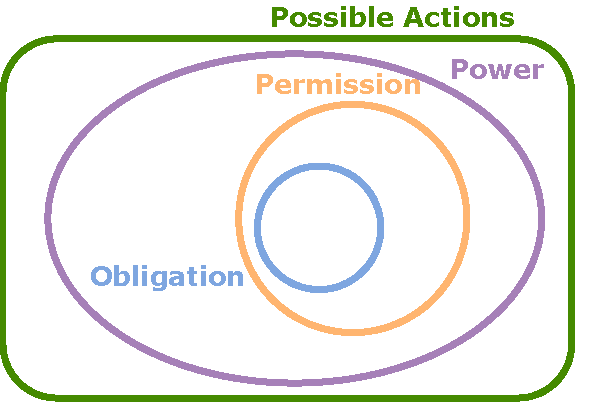
\includegraphics[width=0.6\textwidth]{05_iigo/images/SOMAS_per_obl.pdf}
\caption{Relationship between \emph{power}, \emph{permission} and \emph{obligation}.}
\label{fig:per_obl_sets}
\end{figure}


For example, the Judge has the \emph{power} to carry out investigations at an IIGO session. There are no rules specifying which specific islands the Judge should investigate. Therefore, the Judge has the \emph{permission} to investigate any `alive' islands during a session. However, the Judge is \emph{obliged} to make at least some number of investigations each turn.



\section{Executive Branch}
\label{sec:executive}
The executive branch is responsible for \textbf{carrying out the law}.
\begin{itemize}

    \item The President has the \emph{power} to:
    \begin{itemize}

        \item Select a rule for voting $R^{*}$ to be passed to the Speaker.
        \begin{rule_IIGO}
            The President has the \emph{obligation} to \emph{select} a rule $R^{*}$ if the \emph{rule proposal list} has at least one proposed rule in it.
        \end{rule_IIGO}
        \begin{rule_IIGO}
            The President has the \emph{permission} to \emph{select} a rule $R^{*}$ if and only if $R^{*} \in S$, where $S$ is the \emph{rule proposal list}.
        \end{rule_IIGO}

        \item Decide the amount of individual \emph{taxation} (i.e. a specific \emph{minimum} amount of contribution to the common pool for each island) for the current turn.

        \begin{itemize}
            \item The President is given the self-reported resource amounts held by each island to assist in this decision.
            %\item Suggested Rule: For any island that has chosen to not report it's resources, the President has the \emph{obligation} to set them an individual tax amount T.
        \end{itemize}

        \item Decide the allocation of resources distributed from the common pool to the islands (i.e. a specific \emph{maximum} amount an island is permitted to take from the common pool).

        \begin{itemize}
            \item The President is given the \emph{allocation requests} made by each island.
            %\item \emph{}{Suggested Rule:} The President has an obligation to prioritise islands in critical condition.
        \end{itemize}
    \end{itemize}
\end{itemize}



\section{Legislative Branch}
\label{sec:legislative}
The legislative branch is responsible for \textbf{making the law}.
\begin{itemize}

    \item The Speaker has the \emph{power} to:
    \begin{itemize}

        \item Call a vote $V$ for a rule $R$.
        \begin{rule_IIGO}
            The Speaker has the \emph{obligation} to \emph{call} a vote $V$ if and only if the President has \emph{selected} a rule $R$ to be voted on.
        \end {rule_IIGO}
        \begin{rule_IIGO}
            The Speaker has the \emph{permission} to \emph{call} a vote $V$ for a rule $R$ if and only if the rule $R = R^{*}$, where $R^{*}$ is the rule \emph{selected} by the President.
        \end {rule_IIGO}

        \item Choose which islands are participating in the vote $V$.
       % \footnote{This is our sequential implementation alternative for the power to close the ballot box.}.
        \begin{rule_IIGO}
            The Speaker has the \emph{obligation} to ask for a vote from all alive islands.
        \end {rule_IIGO}

        \item Declare the result $C$ of a vote $V$.
        \begin{rule_IIGO}
            The Speaker has the \emph{obligation} to \emph{declare the result} $C$ for a vote $V$ if and only if the vote V has been \emph{called}.
        \end {rule_IIGO}
        \begin{rule_IIGO}
            The Speaker has the \emph{permission} to \emph{declare the result} $C$ for a vote $V$ if $C = C^{*}$, where $C^{*}$ is the result produced by \emph{calling} the vote $V$.
        \end {rule_IIGO}
        \begin{itemize}
            \item This step is what enables a rule to be \emph{active}.
        \end{itemize}
    \end{itemize}
\end{itemize}




\section{Judicial Branch}
\label{sec:judicial}

The judicial branch is responsible for \textbf{evaluating the law}.
\begin{itemize}
    \item The Judge has the \emph{power} to:
    \begin{itemize}
        \item Perform a number of \emph{inspections}\footnote{An \emph{inspection} \textbf{costs} an expense of resources (See Definition~\ref{def:invst} for more detail).} $I$ and produce a compliance outcome $\mathbb{O}^{*}$\footnote{Note that the compliance outcome $\mathbb{O}^{*}$ considered is a boolean.}.
        %(true: the island has been compliant with the rules in play, false: the island has not been compliant with the rules in play)
        %\begin{itemize}
           % \item For example, to check if the event outcome is \emph{concurrent}\footnote{Again, what is defined as "concurrent"? A clear definition is needed.} with the rules.
        %\end{itemize}
        \begin{rule_IIGO}
            The Judge has the \emph{obligation} to make at least $N$ investigations at each turn.
        \end{rule_IIGO}
        \item Declare the outcome $\mathbb{O}$ of an inspection $I$ to all islands\footnote{This act of broadcasting is especially important for islands to form an opinion about the sanctioned islands accordingly.}.
        \begin{rule_IIGO}
            The Judge has the \emph{obligation} to declare the outcome $\mathbb{O}$ of an inspection $I$ if and only if the inspection $I$ has been performed.
        \end{rule_IIGO}
        \begin{rule_IIGO}
            The Judge has the \emph{permission} to declare the outcome $\mathbb{O}$ of an inspection $I$ if $\mathbb{O} = \mathbb{O}^{*}$, where $\mathbb{O}^{*}$ is the outcome of the inspection $I$.
        \end{rule_IIGO}
        %\item Initiate the removal of the \texttt{President}.
        %\begin{itemize}
            %\item A good Judge would be especially vigilant during \emph{power transfer} regarding the \emph{President} position (see Section~\ref{leg_const} for more detail).
        %\end{itemize}
        \item Invoke economic \textbf{sanctions} (see Section~\ref{sec:sanctions} for more detail).
        \begin{rule_IIGO}
            The Judge has the \emph{obligation} to invoke a sanction $S$ for an island $X$ if and only if an investigation $I$ has an outcome $\mathbb{O}^{*}$ indicating non-compliance, and $I$ is an investigation of an action taken by island $X$.
        \end{rule_IIGO}
        \item Invoke even more severe sanctions in the case of further disobedience to previous sanction(s).
        \begin{rule_IIGO}
            The Judge has the \emph{permission} to invoke a severer sanction $S'$ for an island $X$ if the island $X$ has not fulfilled the requirements of the previous sanction $S$.
        \end{rule_IIGO}
        \item Pardon the islands which are currently sanctioned.
        \begin{rule_IIGO}
            The Judge has the \emph{permission} to revoke any sanction $S$ of an island $X$ at a specific turn.
        \end{rule_IIGO}
    \end{itemize}
\end{itemize}
%(e.g. a new rule that falls under a "sanction" category \hl{[I'm not sure about this being a `new rule` [Ezgi]]}

\subsection{Sanctions}
\label{sec:sanctions}
All sanctions are of economic nature which include:
        \begin{itemize}
            %\item Revoking an island's access to the common pool.
            \item Enforcing an island to contribute a specific amount of resources to the common pool.
            \begin{itemize}
                \item This does not mean that the Judge has the \emph{power} to take resources from an island in order to put them to the common pool -- the island itself is expected to carry out this implication imposed by the sanction itself, otherwise further punishment can be induced by the Judge.
                \item Similarly, \emph{opinion formulation} will follow accordingly whether the island(s) is/are following the implications imposed by the sanction(s).
            \end{itemize}

    \end{itemize}
    Sanctions are the associated penalty that comes with an island breaking a specific rule. The Judge is in full control of the penalties associated with breaking any rules. Once the Judge has specified the score of the penalty associated with each time an island breaks a rule, the cumulative penalties accumulated by the island are then used to determine which \textbf{sanction tier} that each island falls into. The score threshold to determine the boundaries of the sanction tiers are set by the Judge. At each turn of the game, each island is told whether they are being sanctioned, and if so, which \textbf{sanction tier} that they are currently in. The \textbf{sanction tiers} of the non-compliant islands are also broadcasted to the other islands in the archipelago. To summarize, the sanctioning process follows these steps:



    %Sanctions are based on an island breaking a rule. Each rule must therefore have an associated penalty. By default, we set these penalties such that they add $1$ to the total sanction score for each island. However, we allow the judge to override this scoring, the judge is able to set their own scores for any particular rule as they desire. This custom scoring is then used when an island breaks a particular rule. By looking at events that occurred in the last turn, and using the customised scoring we provide the holder of the judge role with full control of the penalties for breaking any rules.







%we then use the cumulative penalties accumulated by each island to determine which Sanction Tier they fall into. The score threshold's required to fall into these sanction tiers is set by the judge and is checked for monotonicity. Each island is told whether they are being sanctioned, and is so what tier they are in. We also tell other islands about which sanction tiers other islands have fallen into.

    \begin{enumerate}
        \item The Judge has the \emph{power} to set custom penalties associated with breaking any rules.
        \item The Judge is given a list of all events that occurred in the previous turn.
        \item The Judge has the \emph{power} to check whether any, or all of these previous events, involve the islands in the archipelago breaking any rules.
        \item Each of the transgressions is scored using the Judge's custom penalties if the Judge has set them. Otherwise, a score of $1$ is given each time a rule is broken.
        \item The Judge has the \emph{power} to revise the sanction thresholds.
        \item Using the latest sanction thresholds available, each island is assigned to a sanction tier based on the sanction score that it has received.
        \item These sanction tiers are broadcasted to all of the islands in the archipelago.
        \item The Judge then uses sanctions rules in place to calculate the specific amount of resources that each non-compliant island has in order to determine how much it should contribute to the common pool, based on the sanction tier that it is in.
    \end{enumerate}



\section{Constitutional Rights and Obligations in the Archipelago}
\label{sec:const_rights_obl_archi}
Each island has the \emph{power} to:
\begin{itemize}
\item make an \emph{allocation request} (see Definition~\ref{def:alloc_req}) to the President for a specific amount to be allocated to them.
\item report the number of resources it is in possession of to the President.
\begin{rule_IIGO}
    Each island has the \emph{obligation} to report the number of resources it is in possession of to the President.
\end{rule_IIGO}
\begin{rule_IIGO}
    Each island has the \emph{permission} to report the number of resources $R'$ if and only if $R' = R$, where R is the number of resources the island is in possession of.
\end{rule_IIGO}
\item take resources from the common pool.


\begin{rule_IIGO}
    Each island has the \emph{permission} to take at maximum $N$ resources, where $N$ is the specific allocation made by the President to that island\footnote{If no such allocation is made, the island is \emph{permitted} to take any amount of resources.}.
\end{rule_IIGO}
\item contribute resources to the common pool.
\begin{rule_IIGO}
    Each island has the \emph{obligation} to contribute to the common pool an amount greater or equal to that of the individual tax set by the President.
\end{rule_IIGO}
                %The President is in
                %(unless there is a rule in place that dictates how Speaker is to allocate resources).
\item add a rule to the \emph{rule proposal list} (see Definition~\ref{def:rule_prop_list}) at the start of each turn.
        %\begin{itemize}
            %\item The game specification includes how many rules an island can propose each turn.
        %\end{itemize}
        %\item vote  for rules in the Legislative Branch and vote for their favourite islands in elections
\item participate in the legislative branch of the government by casting ballots in votes called by the Speaker
\item vote for an island to be elected for a specific role (e.g. the President, Judge, Speaker) during the elections\footnote{This will be assumed to be true \underline{unless stated otherwise}. %Note that \textbf{diplomatic sanctions} can disable this power of a specific island (see Section~\ref{jud_const}).}.
        }.
\end{itemize}
\section{Accountability Cycle}
\label{sec:accountability}

The IIGO roles (i.e. the President, Speaker and Judge) hold a considerable amount of \emph{power}. To ensure that the government is able to avoid corruption and abuse of power, each branch of IIGO is accountable to another through the accountability cycle.
The President is accountable to the Speaker, the Speaker is accountable to the Judge, and the Judge is accountable to the President (see Figure~ \ref{fig:cycles_in_IIGO}). This accountability cycle is enacted through \emph{monitoring} actions\footnote{Note that the terms \textbf{monitoring} and \textbf{investigation} have similar but not identical meanings and different consequences in the context of IIGO.}. The desired effect is for any wrong-doing in IIGO to be determined as quickly as possible and the role in question to be replaced.

The powers related to the accountability cycle and transfer-of-power for each role can be summarized as the following:
\begin{itemize}
    \item The Speaker has the \emph{power} to:
    \begin{itemize}
        \item monitor the President.
        \item declare the result of this monitoring and and if the monitoring result indicates wrongdoing, oblige the Judge to initiate power transfer for the President.
    \end{itemize}
    \item The President has the \emph{power} to:
    \begin{itemize}
        \item monitor the Judge.
        \item declare the result of this monitoring and if the monitoring result indicates wrongdoing, oblige the Speaker to initiate power transfer for the Judge.
    \end{itemize}
    \item The Judge has the \emph{power} to:
    \begin{itemize}
        \item  monitor the Speaker.
        \item declare the result of this monitoring and and if the monitoring result indicates wrongdoing, oblige the President to initiate power transfer for the Speaker.
    \end{itemize}
\end{itemize}

%Unlike investigations performed by the Judge, who performs investigations on island actions in the following turn, each role is given the opportunity to check up on the actions of the role it is responsible for immediately after they have been performed. In this sense, the President can monitor (includes investigative-monitoring) the powers (calling a vote and announcing the result) acted on by the Speaker immediately after the Speaker's announcement (or lack there of). The government officials hold a lot of power so this is to ensure that any wrong-doing is determined as quickly as possible. For this project we are only pursuing one degree of monitoring, that is, the powers relating to the accountability cycle will not be monitored themselves. We assume that agents will act in the interest of themselves and keeping all the islands alive is beneficial to everyone. Hence, while the agents might be inclined to break rules in order to benefit themselves, anyone else breaking the rules is seen as undesirable under the assumption that the system in place is there to benefit all.

The result of monitoring is intended to be a trigger for the initiation of power transfer, whereby a declaration of a negative result indicates that at least one rule was broken by the role monitored and the role should be re-elected. Each turn, in addition to monitoring the actions taken by the role in that IIGO session, the election that role held in the previous IIGO session, if one was held at all, is checked for compliance with the rules of power-transfer.

Figure~ \ref{fig:cycles_in_IIGO} illustrates the reverse nature of the monitoring and power transfer cycles. This is a choice made by design to spread out the process of pre-mature removal from power as a result of wrongdoing. The goal is to avoid malice. If it is one role's power to monitor, it is the other's to initiate and facilitate power transfer. Hence the latter is given a second opinion for cases where the declaration of wrongdoing is not truthful.

Within the scope of the coursework, we decided to pursue only \emph{one degree of monitoring}, meaning that the powers relating to the accountability cycle will not be monitored themselves. We assume that agents will act in the interest of all the islands in the archipelago. Hence, while the agents might be inclined to break the rules to benefit in some form, it is assumed that the others will negatively see any non-compliant islands based on the assumption that the proposed IIGO system is in place to maintain the welfare of all the islands. We still have rules governing this process (see Rule~\ref{rule:monitoring_1} and Rule~\ref{rule:monitoring_2}), however these rules are not enforced.

The \emph{one degree of monitoring} is another justification for the reverse nature of the monitoring and power transfer cycles. The addition of a second opinion means that a role does not hold the power to both wrongfully declare wrongdoing and hold an election for the same role.

Let role $X$ be accountable to the role $Y$, which is accountable to the role $Z$. Then:
\begin{rule_IIGO} \label{rule:monitoring_1}
    $Y$ has the \emph{obligation} to declare the outcome of the monitoring result $M$ associated with the action $A$ undertaken by $X$ if and only if $Y$ has monitored the action $A$ performed by $X$.
\end{rule_IIGO}
\begin{rule_IIGO} \label{rule:monitoring_2}
    $Y$ has the \emph{permission} to declare the monitoring result $M$ associated with the action $A$ undertaken by $X$ if and only if $M = M^{*}$, where $M^{*}$ is the outcome of \emph{monitoring} action $A$ performed by $X$\footnote{These constitutional rules should be available to the agents to check their decisions against. However, due to having only one degree of accountability cycle in place, these rules are not enforced through any sanctions (i.e. breaking these rules has no consequence as they are only deemed to be an \emph{agreement} between the roles).}.
\end{rule_IIGO}


\begin{figure}[!htb]
\centering
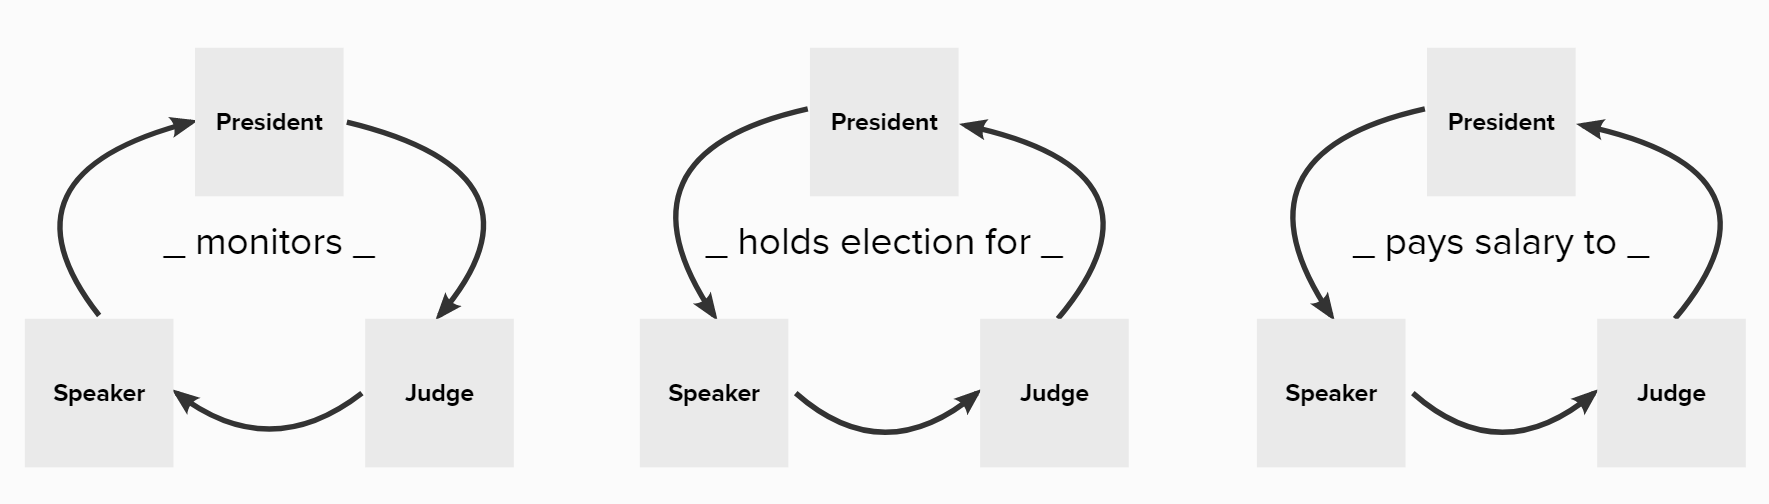
\includegraphics[scale=0.33]{05_iigo/images/role cycles.png}
\caption{Accountability cycle (left), the transfer-of-power cycle (middle) and salary cycle (right).}
\label{fig:cycles_in_IIGO}
\end{figure}


\subsection{Transfer-of-power}
\label{subsec:transfer-of-power}

For the scope of this project, we chose elections to be the only system of power transfer for the islands to utilise. The islands that hold institutional power are the decision group of the archipelago. They decide on taxes, allocations and sanctions. By holding an election for the institutional roles, the islands are not directly included in the decision group, but they do participate in deciding who will occupy these roles and thus who makes the aforementioned decisions. Elections also open up another avenue for opinion formation to have an effect.
\begin{itemize}
    \item Each role has the \emph{power} to call an election vote and declare the winner (see Figure~\ref{fig:cycles_in_IIGO} for the transfer-of-power cycle).
\end{itemize}

We note that:
\begin{enumerate}
    \item The Speaker conducts an election to appoint a new Judge.
    \item The Judge conducts an election to appoint a new President.
    \item The President conducts an election to appoint a new Speaker.
\end{enumerate}
Refer to the Figure~ \ref{fig:cycles_in_IIGO} for further clarification about the transfer-of-power cycle.

We introduce a \emph{term} length to increase the diversity of the decision group. If the Rule~\ref{rule:roles_must_hold_election} is in play, the roles are obliged to hold an election every $N$ turns. To reduce the scope of the coursework, the term length is defined as a configuration parameter. Thus we reduce the complexity of rules surrounding the election of roles and hence the reasoning the agents have to do with regard to said rules.

\begin{rule_IIGO} \label{rule:roles_must_hold_election}
    The role $X$ has the \emph{obligation} to conduct a vote for the election of $Y$ if and only if $Y$ has been in power for more turns than the turn length or if role $Z$ has made a monitoring announcement that indicates wrongdoing by $Y$
\end{rule_IIGO}

\begin{rule_IIGO} \label{rule:must_appoint_elected_island}
    The role $X$ has the \emph{permission} to \emph{declare the winner} $W$ for an election $E$ if $W = W^{*}$, where $W^{*}$ is the winner produced by \emph{calling} a vote for the election $E$.
\end {rule_IIGO}

Unlike the rule vote held by the Speaker, the process of election is more regimented. The power of calling a vote for an election and the power of declaring the result are combined into one action. This decision came as a result of a motion to simplify the system for implementation. However, the powers are still kept somewhat separate. When facilitating an election, the roles still have the option to declare a winner of their choosing. Rule~\ref{rule:must_appoint_elected_island} is what governs this choice. However, the agents do not have the option to not declare a result at all: holding an election will always result in a declaration of the winner.

\section{Budget and Salary}
\subsection{Budget}
%Actions associated with the IIGO have an associated cost that is defined as a configuration parameter. The institutional-power-enabled actions of  identified to require a "computational" component are:

For the simulation we have defined the resources gathered by the islands to be endogenous. Hence we assume that self-organization will consume those resources and institutional-power-enabled actions in the IIGO have an associated cost. The institutional-power actions with such a cost are:


%that is defined as a configuration parameter. The institutional-power-enabled actions of  identified to require a "computational" component are:


%We have defined the resource to be an endogenous one, hence any computation surrounding the distribution of the resource must use up some of that resource.
\begin{itemize}
\item President selecting a rule from the rule proposal list.
\item President deciding the amount of individual taxation.
\item President deciding the allocation of resources from the common pool.
\item Speaker calling a vote and calculating the winner.
\item Judge inspecting an island's actions.
\item Judge inspecting an island's action history retroactively.
\item Declaring (e.g. \textit{announcing} the result of a vote).
\item Holding an election.
\item Monitoring a role.
\end{itemize}

IIGO has been designed to act in the common good. Therefore IIGO-related costs will be directly withdrawn from the common pool. Since the common pool is considered communal property of the archipelago, there are rules in place to limit how much each role is allowed to spend in order to perform its own institutional-power-enabled actions. This is the reason for defining the \emph{budget} and keeping it separate for each of the three IIGO roles.

\begin{rule_IIGO} \label{rule:budget}
    %Each role has the \emph{obligation} to pay the salary of amount $S$ to another if and only if the amount paid $S'$ is equal to $S$.
    Each role has the \emph{permission} to act on an institutional-power action with an associated cost if the budget would not become negative as a result of performing the action.
 \end{rule_IIGO}



When a role acts on an institutional-power-enabled action with a cost, the cost associated with this action is subtracted from the role's \emph{budget}. If Rule~\ref{rule:budget} is in play, a budget of zero or less means that the role does not have the \emph{permission} to perform any of its institutional-power actions. The removal of Rule~\ref{rule:budget} from the rules in play means the role is permitted to perform as many such actions as it would like (as long as those actions are not governed by other rules).

The \emph{budget} is persistent across turns. This means that, assuming nothing else affects the budget, if a role has $100$ resources in its budget at the start of a turn and spends $10$ resources, the same role has $90$ resources in its budget at the start of next turn. On the other hand, islands can choose to increase the budget periodically at every turn. The islands can choose the magnitude of this periodic increase by voting on a rule.

%one turn and it spends 10, it has 90 resources in it's budget the next turn.

Finally, it must be noted that the budget is inherently linked with  whether the obligations of a specific role can be undertaken.
For example, during \emph{monitoring}, it is not seen to be a rule violation if a role has not acted on an obligation as doing so would require it to go over budget.

%This can also be seen as an added clause "... and the action is only permitted if they have the budget" to most rules which govern actions with an endogenous-cost.
%\begin{rule_IIGO}
    %The budget is increased by an amount $N$ every turn.
%\end{rule_IIGO}

%This rule means that, assuming nothing else affects the budget, if a budget is set to increase by 10 resources every turn and the budget is a 100 resources in turn one, the budget is 110 resources in turn 2. Setting this rule to 0 is equal to removing this rule and it means that the budget is never increased.


\subsection{Salary}
\label{subsec:salary}
A salary is paid to each role in power as an incentive to be in power. Since our system has regimented the means of power transfer to be an election, this incentive extends to acting in a publicly approved way. %Hence, each role has the \emph{power} to pay a salary to another role following the salary cycle in Figure~\ref{fig:cycles_in_IIGO}.
\begin{rule_IIGO} \label{rule:salary}
   Each role has the \emph{obligation} to pay the salary of amount $S$ to one another following the salary cycle in Figure~\ref{fig:cycles_in_IIGO}.
\end{rule_IIGO}

In Rule~\ref{rule:salary}, setting $S=0$ (through changing the active rules in place) means that roles do not have the permission to pay any salary. Removing the Rule~\ref{rule:salary} means that the roles may freely choose the amount $S$ for the salary payments.

\section{IIGO Session Order}
Each IIGO Session can be broken down into a sequence of consecutive actions by the Judiciary, Executive and Legislature. The session is concluded with monitoring, salary payments and elections.
\subsection{Judicial Actions}
\begin{enumerate}
    \item The Judge has the \emph{power} to check the history of actions to confirm whether the previously punished island(s) has/have obeyed the previous round's sanctions, meaning whether they contributed to the common pool accordingly in case of economic sanctions.
    %\begin{itemize}
      %  \item \emph{Suggested Rule:} In case of disobeying sanctions, the Judge is \emph{obliged} and \emph{permitted} to increase the severity of sanctions with respect to specific islands.
   % \end{itemize}
    \item The Judge has the \emph{power} to carry out \emph{inspections} on the history of actions of any island $X$ to check whether:
        \begin{enumerate}
        \item the reported resources of $X$ in the previous round match the real value of resources $X$ had in its private pool for the previous turn.
        \item the island $X$ has retrieved the right amount of the resources from the common pool, based on the \emph{allocation request} evaluated by the previous President.
            \begin{itemize}
            \item An example: In the previous round, the President has decided that the island $X$ can take $Y$ amount of resources from the common pool. If the Judge finds out that the island $X$ has taken an amount of $Y'$ such that $Y' > Y$, the Judge has the \emph{power} to invoke sanctions on the island $X$.

            %the Judge is \emph{obliged} and \emph{permitted} to sanction island $X$.
            \end{itemize}
        \end{enumerate}
    \item The Judge has the \emph{power} to invoke sanctions based on the outcome of the inspections.
\end{enumerate}
\subsection{Executive Actions}
\begin{enumerate}
    \item The islands may report the resources in their private pools to the President.
    \item The President has the \emph{power} to let each island know about the amount of \emph{taxation} they have to pay.
    \item The island has the \emph{power} to make an \emph{allocation request} to the President.
    \item The President has the \emph{power} decide on an allocation of resources and let each island know about the amount of resource allocation they are permitted to take from the common pool.
    \item The island has the \emph{power} to pick and to propose a rule to be voted on to the President.
    \item The President has the \emph{power} to choose a rule to be voted on from the received rule proposals.
\end{enumerate}
\subsection{Legislative Actions}
\begin{enumerate}
    \item The Speaker has the \emph{power} to call a vote.
        \begin{enumerate}
        \item The islands vote in support of, or against, the rule (aye or nay) anonymously.
        \end{enumerate}
    \item The Speaker has the \emph{power} to announce a result of a vote to the islands and carries out the law change, if required (e.g. deleting/rejecting a rule if there is a majority nay vote).
\end{enumerate}
\subsection{End of Session Actions}
\begin{enumerate}
    \item The roles pay a salary to one another following the accountability cycle in Figure~ \ref{fig:cycles_in_IIGO}.
    \item The Speaker has the \emph{power} to decide to carry out \emph{monitoring} on:
    \begin{enumerate}
    \item the resource allocation decided by the President.
    \item the rule proposed by the President.
    \item the previous IIGO session's election for a new Speaker, if an election was held.
    \end{enumerate}
    \item The President has the \emph{power} to decide to carry out \emph{monitoring} on:
    \begin{enumerate}
        \item the sanctions imposed by the Judge.
        \item the previous IIGO session's election for a new President, if an election was held.
    \end{enumerate}
    \item The Judge has the \emph{power} to decide to carry out \emph{monitoring} on:
    \begin{enumerate}
        \item the vote called by the Speaker.
        \item the Speaker announcing the result.
        \item the previous IIGO session's election for a new Judge, if an election was held.
    \end{enumerate}
    \item The Speaker has the \emph{power} to decide to hold an election for a new Judge.
    \item The President has the \emph{power} to decide to hold an election for a new Speaker.
    \item The Judge has the \emph{power} to decide to hold an election for a new President.
\end{enumerate}



\section{Future Work}

\begin{itemize}
    \item \textbf{Diplomatic sanctions}: Although having the potential of being a good alternative for severer sanctions discussed in  Section~\ref{sec:sanctions}, diplomatic sanctions are \emph{not} implemented within the scope of the coursework. \\
    Suggested diplomatic sanctions include:
        \begin{itemize}
            \item Revoking an island's eligibility to vote and to be elected for a position.
            \item Revoking an island's eligibility to propose a rule/motion.
        \end{itemize}
    \item \textbf{Immutable rules}: Within the scope of the coursework, a subset of rules could have been categorised as immutable. This means that to change such immutable rules, the islands first need to vote to change their status to be \emph{mutable}, and consequently, hold another vote to change these mutable rules.
    %\item \textbf{Adding rules to the proposal list: }
\end{itemize}
